%------------------------------------------
%       $Id$
%
%       The GMT Documentation Project
%	Copyright (c) 2000-2013.
%	P. Wessel, W. H. F. Smith, R. Scharroo, J. Luis and F. Wobbe
%------------------------------------------
%

%----------------------ACKNOWLEDGMENTS--------------------------

\chapter*{Acknowledgments}\index{Acknowledgments}
\addcontentsline{toc}{chapter}{Acknowledgments}

The Generic Mapping Tools (\GMT) could not have been designed without
the generous support of several people.  We gratefully acknowledge
A. B. Watts and the late W. F. Haxby for supporting our efforts on the original
version 1.0 while we were their graduate students at Lamont-Doherty
Earth Observatory.  Doug Shearer and Roger Davis patiently answered
many questions over e-mail.  The subroutine \texttt{gauss}
was written and supplied by Bill Menke.
Further development of versions 2.0--2.1 at SOEST would not have
been possible without the support from the HIGP/SOEST
Post-Doctoral Fellowship program to Paul Wessel.  Walter H. F. Smith
gratefully acknowledges the generous support of the C. H. and I. M.
Green Foundation for Earth Sciences at the Institute of Geophysics
and Planetary Physics, Scripps Institution of Oceanography, University
of California at San Diego.
\GMT\ series 3.x, 4.x, and 5.x owe their existence to grants
EAR-93-02272, OCE-95-29431, OCE-00-82552, OCE-04-52126, and OCE-1029874
from the National Science Foundation, which we gratefully acknowledge.

We would also like to acknowledge feedback, suggestions and bug reports
from
Michael Barck,
Manfred Brands,
Allen Cogbill,
Stephan Eickschen,
Ben Horner-Johnson,
John Kuhn,
Angel Li,
Andrew Macrae,
Alex Madon,
Ken McLean,
Greg Neumann,
Ameet Raval,
Georg Schwarz,
Richard Signell,
Peter Schmidt,
Dirk Stoecker,
Eduardo Su\'{a}rez,
Mikhail Tchernychev,
Malte Thoma,
David Townsend,
Garry Vaughan,
William Weibel,
and many others, including their advice
on how to make \GMT\ portable to a wide range of platforms.
John Lillibridge and Stephan Eickschen provided the original examples 11 and 32, respectively;
Hanno von Lom helped resolve early problems with DLL libraries for Win32;
Lloyd Parkes enabled indexed color images in \PS;
Kurt Schwehr maintains the \textsf{Fink} packages;
Wayne Wilson implemented the full general perspective projection;
and William Yip helped translate \GMT\ to POSIX ANSI C and incorporate netCDF 3.
The SOEST RCF staff (Ross Ishida, Pat Townsend, and Sharon Stahl) provided valuable help
on Linux, web, and CGI script issues.

\begin{flushright}
Honolulu, HI, Silver Spring, MD, Cornish, NH, Faro, Portugal, and Bremerhaven, Germany \GMTDOCDATE
\end{flushright}

\noindent
\begin{figure}[H]
	\centering
	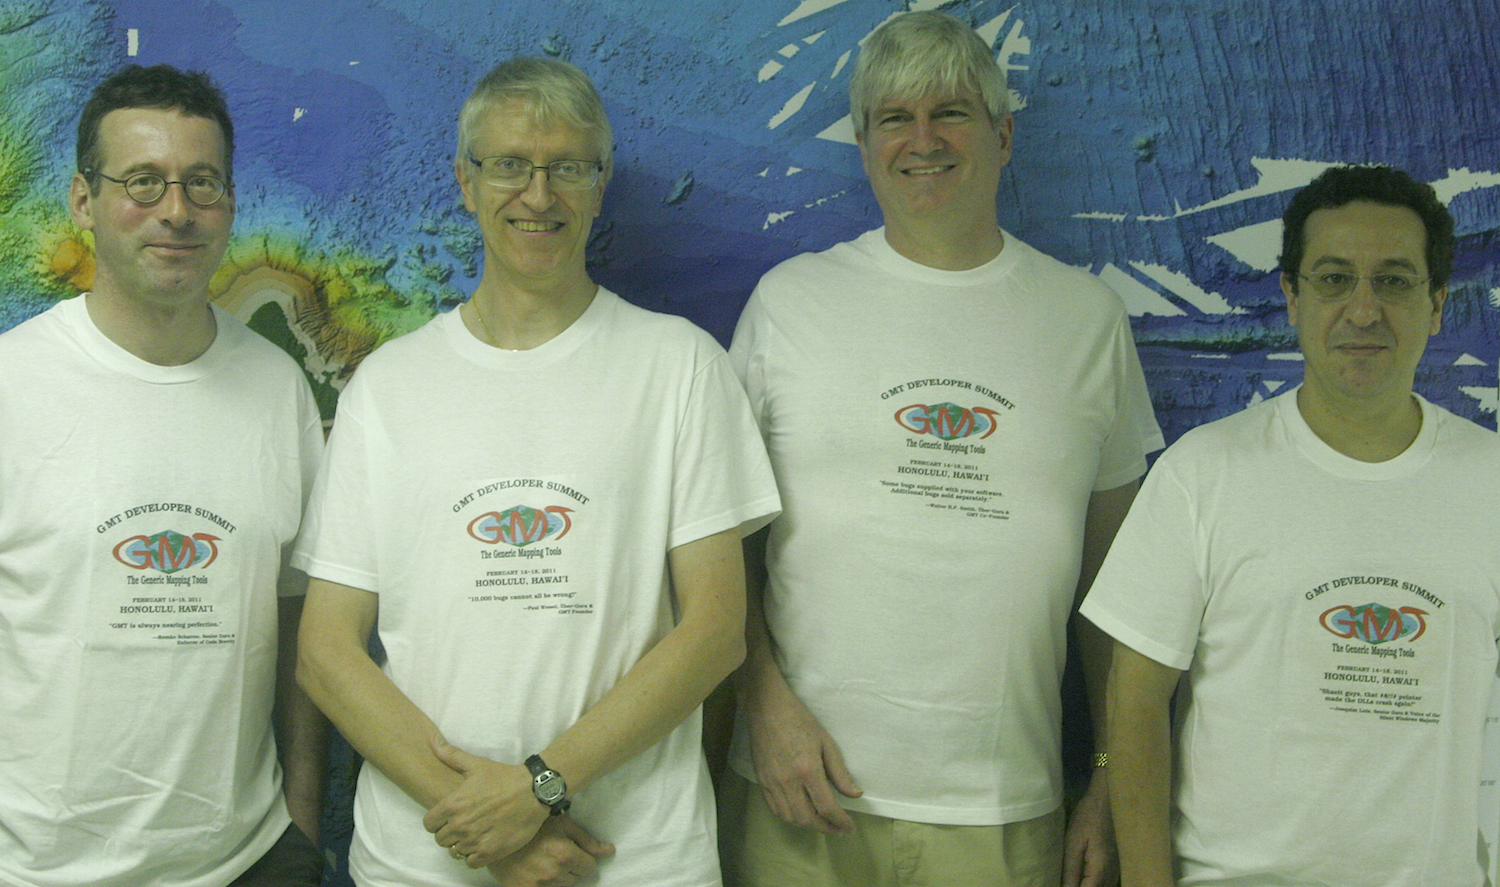
\includegraphics[width=\textwidth]{GMT5_Summit_2011.png}
	\caption{The four horsemen of the \GMT\ apocalypse: Remko Scharroo, Paul Wessel,
	Walter H.F. Smith, and Joaquim Luis at the \GMT\ Developer Summit in Honolulu,
	Hawaii during February 14--18, 2011.  Since then a fifth horseman, Florian Wobbe, has
	been added to the stable.}
\end{figure}

%------------------------GMT DOCUMENTATION PROJECT---------------------------

\chapter*{The GMT Documentation Project}
\addcontentsline{toc}{chapter}{The GMT Documentation Project}

Starting with \GMT\ version 3.2, all \GMT\ documentation was
converted from Microsoft \progname{Word} to \LaTeX\ files.
This step was taken for a number of reasons:

\begin{enumerate}

\item Having all the documentation source available in
ASCII format makes it easier to access by several
\GMT\ developers working on different platforms in 
different countries.

\item \GMT\ scripts can now be included directly into the text
so that the documentation is automatically up-to-date
when scripts are modified.

\item All figures are generated on the fly and included as
\GMT\ EPS files which thus are always up-to-date.

\item It is easy to convert the \LaTeX\ files to other
formats, such as HTML, SGML, \PS, and PDF.

\item The whole task of assembling the pieces, be it generating
figures or extracting text portions from the master archive under
Subversion control, is automated by a makefile.

\item Only free software are used to maintain the \GMT\ Documentation.

\end{enumerate}

Please send email to
\htmladdnormallink{the GMT help list}{mailto:gmt-help@lists.hawaii.edu}
(subscription required; see Appendix D) if you find errors or inconsistencies in the documentation.
%--------------------------------REMINDER------------------------------------

\chapter*{A Reminder}
\addcontentsline{toc}{chapter}{A Reminder}

If you feel it is appropriate, you may consider paying us back by
citing our \emph{EOS} articles on \GMT\ (and perhaps also our Geophysics
article on the \GMT\ program \GMTprog{surface}) when you publish papers
containing results or illustrations obtained using \GMT.  The EOS
articles on \GMT\ are
\index{EOS article}%
\index{Article!in EOS}%

\begin{itemize}

\item{Wessel, P., and W. H. F. Smith, New, improved version of Generic
Mapping Tools released, \emph{EOS Trans. Amer. Geophys. U.}, vol. 79
(47), pp. 579, 1998.}

\item{Wessel, P., and W. H. F. Smith, New version of the Generic
Mapping Tools released, \emph{EOS Trans. Amer. Geophys. U.}, vol. 76
(33), pp. 329, 1995.}

\item{Wessel, P., and W. H. F. Smith, New version of the Generic
Mapping Tools released, \emph{EOS Trans. Amer. Geophys. U. electronic
supplement}, \htmladdnormallink{http://www.agu.org/eos\_elec/95154e.html}
{http://www.agu.org/eos\_elec/95154e.html}, 1995.}

\item{Wessel, P., and W. H. F. Smith, Free software helps map and
display data, \emph{EOS Trans. Amer. Geophys. U.}, vol. 72 (41),
pp. 441, 445-446, 1991.}

\end{itemize}
\noindent
Some \GMT\ programs are based on algorithms we have developed and
published, such as

\begin{itemize}

\item Kim, S.-S., and P. Wessel, Directional Median Filtering for Regional-Residual
Separation of Bathymetry, \emph{Geochem. Geophys. Geosyst., 9(Q03005)}, doi:10.1029/2007GC001850.
[\GMTprog{dimfilter.c} in \GMTprog{misc} supplement].

\item Smith, W. H. F., and P. Wessel, Gridding with Continuous
Curvature Splines in Tension, \emph{Geophysics}, vol. 55 (3), pp.
293--305, 1990 [\GMTprog{surface.c}].

\item Wessel, P., A General-purpose Green's Function-based Interpolator,
\emph{Computers \& Geosciences}, vol. 35, pp. 1247--1254, 2009  [\GMTprog{greenspline.c}].

\item  Wessel, P., Tools for Analyzing Intersecting Tracks: the x2sys package,
\emph{Computers \& Geosciences}, vol. 36, 348--354, 2010  [\GMTprog{x2sys} supplement].

\item Wessel, P. and J. M. Becker, Interpolation using a Generalized
Green's Function for a Spherical Surface Spline in Tension,
\emph{Geophys. J. Int.}, vol. 174, pp. 21--28, 2008  [\GMTprog{greenspline.c}].

\end{itemize}

\noindent
Finally, \GMT\ includes some code supplied by others, in particular the Triangle code
used for Delaunay triangulation.  Its author, Jonathan Shewchuk, says
\begin{quote}
``If you use Triangle, and especially if you use it to accomplish real
work, I would like very much to hear from you.  A short letter or email
(to jrs@cs.cmu.edu) describing how you use Triangle will mean a lot to
me.  The more people I know are using this program, the more easily I can
justify spending time on improvements and on the three-dimensional
successor to Triangle, which in turn will benefit you.''
\end{quote}

A few \GMT\ users take the time to write us letters, telling us of the
difference \GMT\ is making in their work.  We appreciate receiving these
letters.  On days when we wonder why we ever released \GMT\ we pull
these letters out and read them.  Seriously, as financial support for
\GMT\ depends on how well we can ``sell'' the idea to funding agencies and
our superiors, letter-writing is one area where \GMT\ users can affect
such decisions by supporting the \GMT\ project. 

%-------------------------COPYRIGHT----------------------------------

\chapter*{Copyright and Caveat Emptor!}
\index{Copyright}
\addcontentsline{toc}{chapter}{Copyright and Caveat Emptor!}

\begin{center}
Copyright \copyright 1991 -- \GMTDOCYEAR\ by P. Wessel, W. H. F. Smith, R. Scharroo, J. Luis and F. Wobbe
\end{center}

\vspace{\baselineskip}

The Generic Mapping Tools (\GMT) is free software; you can redistribute
it and/or modify it under the terms of the GNU Lesser General Public License
as published by the Free Software Foundation. \\

The \GMT\ package is distributed in the hope that it will be useful, but
WITHOUT ANY WARRANTY; without even the implied warranty of
MERCHANTABILITY or FITNESS FOR A PARTICULAR PURPOSE.  See the
file \filename{LICENSE.TXT} in the \GMT\ directory or the
\htmladdnormallinkfoot{GNU Lesser General Public License}{http://www.gnu.org/licenses/lgpl.html}
for more details. \\

Permission is granted to make and distribute verbatim copies of this
manual provided that the copyright notice and these paragraphs are
preserved on all copies.  The \GMT\ package may be included in a bundled
distribution of software for which a reasonable fee may be charged. \\

The Generic Mapping Tools (\GMT) does not come with any warranties,
nor is it guaranteed to work on your computer.  The user assumes full
responsibility for the use of this system. In particular, the University
of Hawaii School of Ocean and Earth Science and Technology, the National
Oceanic and Atmospheric Administration, Altimetrics LLC, the Universidade
do Algarve, Alfred Wegener Institute, the National Science Foundation,
Paul Wessel, Walter H. F. Smith, Remko Scharroo, Joaquim F. Luis, Florian
Wobbe or any other individuals involved in the design and maintenance of
\GMT\ are NOT responsible for any damage that may follow from correct
\emph{or} incorrect use of these programs.

%----------------------TYPOGRAPHIC CONVENTIONS------------------------

\chapter*{Typographic conventions}
\index{Typographic conventions}
\addcontentsline{toc}{chapter}{Typographic conventions}

In reading this documentation, the following provides a summary of
the typographic conventions used in this document.

\begin{enumerate}

\item User input and \GMT\ or \UNIX\ commands are indicated by
using the \texttt{typewriter} type style, e.g., \texttt{chmod +x job03.sh}.

\item The names of \GMT\ programs are indicated by the
\textsfbf{bold, sans serif} type style, e.g., we plot text with \textsfbf{pstext}.

\item The names of other programs are indicated by the
\textslbf{bold, slanted} type style, e.g., \textslbf{grep}.

\item File names are indicated by the \underline{underline}
type style, e.g., \underline{gmt.h}.

\end{enumerate}
